\documentclass[10pt,twocolumn,letterpaper]{article}

\usepackage{cvpr}
\usepackage{times}
\usepackage{epsfig}
\usepackage{graphicx}
\usepackage{amsmath}
\usepackage{amssymb}

% point to the figures
\graphicspath{ {images/} }

% Include other packages here, before hyperref.

% If you comment hyperref and then uncomment it, you should delete
% egpaper.aux before re-running latex.  (Or just hit 'q' on the first latex
% run, let it finish, and you should be clear).
\usepackage[breaklinks=true,bookmarks=false]{hyperref}

\cvprfinalcopy % *** Uncomment this line for the final submission

\def\cvprPaperID{****} % *** Enter the CVPR Paper ID here
\def\httilde{\mbox{\tt\raisebox{-.5ex}{\symbol{126}}}}

% Pages are numbered in submission mode, and unnumbered in camera-ready
%\ifcvprfinal\pagestyle{empty}\fi
\setcounter{page}{1}
\begin{document}

%%%%%%%%% TITLE
\title{A Low Cost Eye-tracking Interface to Help the Physically
  Impaired Users}

\author{Thomas Karpat (SCPD)\\
Stanford University \\
{\tt\small tkarpati@stanford.edu}
% For a paper whose authors are all at the same institution,
% omit the following lines up until the closing ``}''.
% Additional authors and addresses can be added with ``\and'',
% just like the second author.
% To save space, use either the email address or home page, not both
\and
Shankar Thadhalani (SCPD)\\
Stanford University \\
{\tt\small shankart@stanford.edu}
}

\maketitle
%\thispagestyle{empty}

%%%%%%%%% ABSTRACT
\begin{abstract}
This paper presents a low cost alternative to traditional eye-tracking
interface to help physically impaired users interact. We propose to
implement an eye-tracking system utilizing a single camera. We present a
Convolutional Neural Networks based approach which eliminates the
necessity of external light source as required by existing solution.
\end{abstract}

%%%%%%%%% BODY TEXT
\section{Introduction}
We propose to implement an eye-tracking system utilizing a single
camera. Gaze tracking has numerous application in human computer
interfaces from use as input for the impaired\cite{calvo}, to
determination of region of interest for augmented reality and image
processing. Our system would use a camera on a laptop and determine
the target of the users gaze. This would then be used to move a cursor
around a graphical keyboard on the display which could be used for
input. Our design results in a multi-segment system. We propose to
first segment the face from the image. Then the left and right eyes
are each segmented from the face. The eyes are then fed into a trained
neural network to determine the location of focus for the user. We
will examine work that has already been done in the past on gaze
tracking to build upon. The literature contains systems from strictly
classical approaches to systems that are built on neural networks for
the processing \cite{krafka} \cite{mcmurrough} \cite{weidenbacher}
\cite{baluja} \cite{cazzato} \cite{li}. We hope to be able to use a
combination of the two to achieve good results. While existing
commercial solutions use external light source and additional hardware
to implement eye tracking, we expect to utilize openly available gaze
eye-tracking dataset to eliminate the requirement for any additional
hardware.

\section{Problem Statement}
The existing commercial solution available require external hardware
being attached to existing device\cite{eyetrackerlist}\cite{tobii_1} This makes eye tracking an
expensive and unreachable solution for many. These solutions are based
on external infrared light source and rely on the reflection of the
light from the user’s pupil to identify point of user interest. We hope to
utilize the built in web camera of our system and eliminate the necessity
of additional hardware such as external light sources with help of a
well trained convolutional neural network.

\begin{figure}
  \begin{center}
    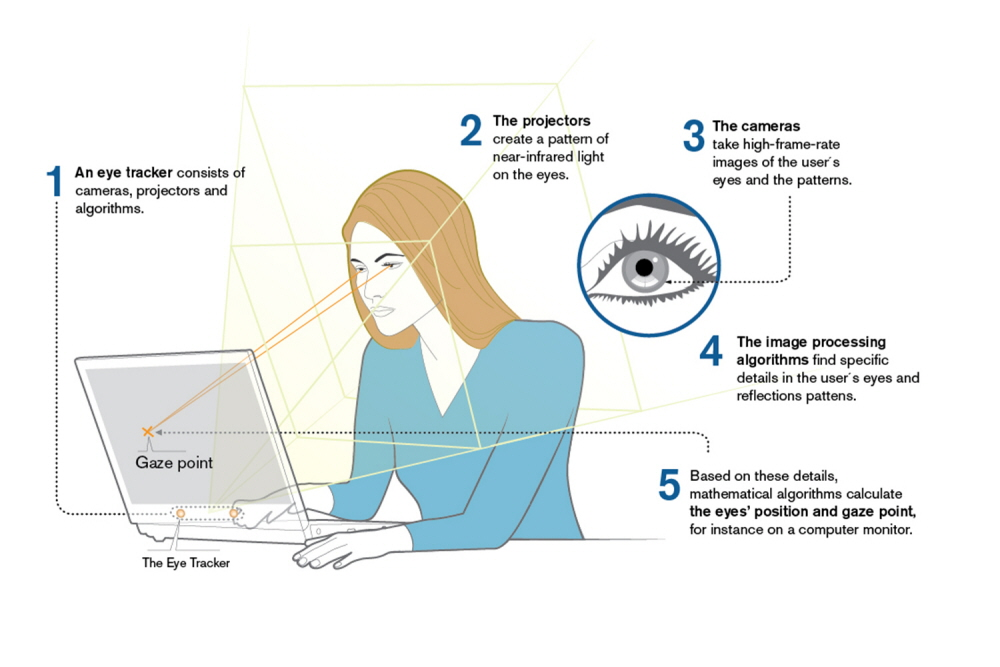
\includegraphics[width=\linewidth]{existing_solutions}
  \end{center}
  \caption{Existing solutions to gaze-tracking problem}
  \label{fig:existsol}
  \end{figure}

A brief introduction of existing solution mechanism can be seen Figure~\ref{fig:existsol}.

\section{Technical Approach}
The system is designed to run 2 threads, one thread to capture 
and validate input from webcam and another to process the 
captured input. The second thread processes the captured and 
sanitized input through our convolutional neural network and 
obtains the point of user interest on the screen. In following section 
we explain the break down of system from image capturing 
to evaluating point of interest.  

\subsection{Image capture and face/eye detection}
We implemented the system in Python 2.7 using the OpenCV libraries for 
image processing tasks. The use of OpenCV gives us an easy hardware 
abstraction layer to video capture and display peripherals. We use 
haar-cascade utilizing Viola-Jones face recognition algorithm to 
identify face and eyes. 

First we capture input stream using peripheral
interface provided by OpenCV. We convert each 
frame as it is captured to grayscale, this frame is then analyzed 
using haar-feature based cascade classifier to identify a face. 
Once we have detected a face, we process frame detected 
as face again using haar-feature based classifier to identify eyes. 

In our initial runs we encountered difficulties with these cascade classifiers.
This can be seen in  (Figure~\ref{fig:defensive}).
In order to sanitize the inputs passed to our neural network, we added 
additional defensive coding to eliminate false positive detection 
for eyes or faces. We make sure a detected face has eyes 
and location of the eyes are not in the lower half of the detected face

\begin{figure}
  \begin{center}
    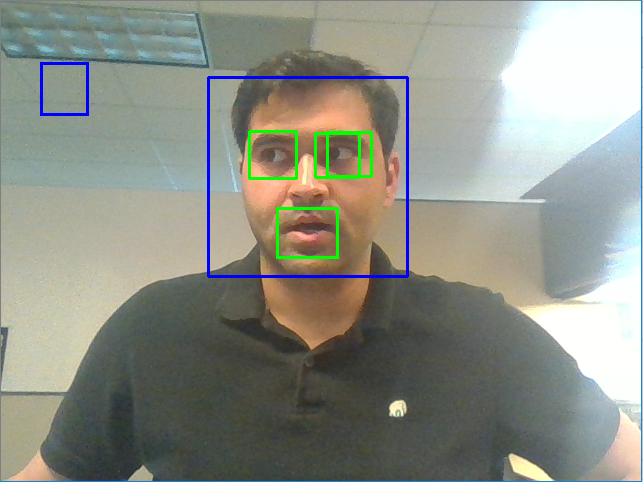
\includegraphics[width=\linewidth]{defensive_coding_example}
  \end{center}
  \caption{Failure observed without defensive coding for face and eye
    verification.}
  \label{fig:defensive}
\end{figure}


Once the face itself has been extracted from the video and the eyes
are isolated from the face, then images  of the face and the location
of eyes are fed into a neural network to determine the location of the
gaze.


\subsection{Neural Network}
The neural network is implemented in TensorFlow. The neural network is
a multilayer classifier where the inputs are the extracted images of
the eyes and the bounding boxes for the eyes and the face in the
original image. The two images of the eyes are 32x32x3 images where
the extracted images of the eyes are scaled to a set size. This gives
us a fixed image size to feed into the network invariant of the
original size of the eyes in the original video frame. The size of
32x32 should be large enough to provide enough detail without creating
a network that is too large. It is in line with work that has come
before.

\begin{figure}
  \begin{center}
    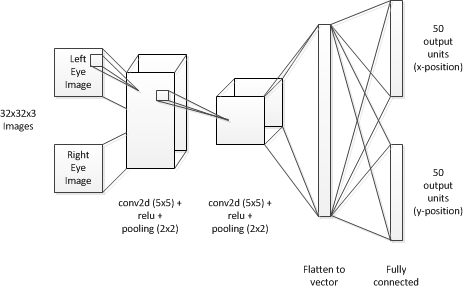
\includegraphics[width=\linewidth]{gaze-tracking-cnn-arch}
  \end{center}
  \caption{Neural Network Architecture}
  \label{fig.cnn-arch}
\end{figure}


The images are fed into a bank of 16xs convolutional
filters. This results in an output of 32x32x16 outputs. The filter
kernels have support of 5 pixels in the x- and y-axes. The output of
the convolutional filters is passed through a rectified linear
activation function. Following the convolution layer, we perform max pooling with a
non-overlapping 2x2 filter to reduce the dimentionality.

A second bank of convolutional filters is then convolved with the
output of the first bank. The second set of layers is also a
convolution and max pooling layer. The input of the second bank has
shape of 16x16x16 inputs. The second bank has 16 input and 32 output
channels and stride of 1. The filter kernel has support of 5
pixels. This is essentially the same as the first layer with a
rectified linear activation function, but the dimentionality is
smaller in the image x- and y-axes, and larger in the filter bank
depth. The output again is passed through a max-poolong layer.

Following the two convolutional layers, the output is flattened into a
single vector and passes through a fully connected layer of 200
units. This layer is then connected to two 50 unit output layers in
fully connected fashion. These two sets of 50 units represent the x-
and y- outputs of the gaze. The two sets of 50 output represent
segmenting the angle of gaze into 50 segments where the center output
unit represents a gaze of 0 degrees. The x- and y- axes are separate
here and the output is a softmax function and represents the
probability distribution of the output in the x- and y- directions.

\section{Neural Network Datasets}
We will use the Point of Gaze Eye-Tracking Dataset from the University
of Texas at Arlington\cite{eyetracking}. This provides a mapping from
a video of eyes to locations in 3D space where the gaze of a user is
focusing their attention. The dataset consists of data captured from
20 subjects. The dataset for each subject consists of a video of the
user’s eye, transform matrices that relate the user’s eye and the
screen of a display, and the target location on the screen that the
subject is looking at. There are 6 scenarios for each of the 20
users. The transform and the target locations are provided per frame
of the video. We also plan on using the comprehensive head pose and
gaze database\cite{mcmurrough} to infer correlation between the pose
of the head and the target that the subject is looking at.

We hope to run the system in a real-time manner and compare our
results to expected locations on the display. In this setup data that
we capture from the camera connected to the system will be used as our
system inputs and data to process.

\section{Progress}
Despite some initial hurdles, we are still on track in terms of milestones 
we had initially set for ourselves. We are yet to build test framework 
to evaluate our solution. The test framework is conceptualized 
in the Evaluation section of this report.

\subsection{Neural Network}
We currently have the neural network implemented in TensorFlow, but
has not been trained yet with our dataset.

\subsection{Timeline}
\begin{itemize}
  \item 2/9/18 - Familiarize with opencv and setup base infrastructure for face/eye detection
  \item 2/16/18 - Face and Eye Detection
  \item 2/23/18 - Setup a neural network with existing database
  \item 2/26/18 - Compile and submit progress report
  \item 3/9/18 - Trained the neural network ready for inference 
  \item 3/16/18 - Generate results and demo
\end{itemize}

\begin{figure}
  \begin{center}
    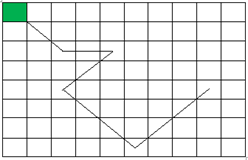
\includegraphics[width=\linewidth]{original_object_path}
  \end{center}
  \caption{Path followed by Object on Screen.}
  \label{fig:originalpath}
\end{figure}

\section{Evaluation}
We propose to evaluate our results by having the user follow an object
around the screen on a known path (Figure~\ref{fig:originalpath}). 
This would be our target. We can then compute the gaze of the user from 
the observations by the system (Figure~\ref{fig:generatedpath}). 
We can compute the error between the computed target from the
gaze of the user and the known target location. From these two
measurements we can compute the mean squared error between the target
and the computed gaze location. We hope to achieve results that are
within the size of the panels used for a keyboard on the screen. If
the error is within the size of a key, then we can determine what keys
a user is looking at, and even use the system as an input device.


\begin{figure}
  \begin{center}
    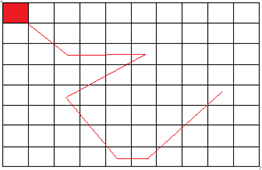
\includegraphics[width=\linewidth]{predicted_object_path}
  \end{center}
  \caption{Path generated by tracking user’s eye.}
  \label{fig:generatedpath}
\end{figure}



{\small
\bibliographystyle{ieee}
\bibliography{egbib}
\begin{thebibliography}{1}
\bibitem{calvo}
  Calvo A. et al.. Eye Tracking Impact on Quality-of-Life of ALS
  Patients. In: Miesenberger K., Klaus J., Zagler W., Karshmer
  A. (eds) \underline{Computers Helping People with Special Needs. ICCHP
    2008}. \underline{Lecture Notes in Computer Science}, vol 5105. Springer,
  Berlin, Heidelberg, 2008
\bibitem{eyetracking}
  http://heracleia.uta.edu/~mcmurrough/eyetracking/
\bibitem{krafka}
  Krafka, Kyle, et al. Eye tracking for everyone.
  \textit{IEEE Conference on Computer Vision and Pattern Recognition
    (CVPR)}, 2016
\bibitem{mcmurrough}
  McMurrough, Christopher D., et al. "A dataset for point of gaze
  detection using head poses and eye images."
  \textit{Journal on Multimodal User Interfaces 7.3} (2013): 207-215.
\bibitem{weidenbacher}
  Weidenbacher, U.; Layher, G.; Strauss, P.-M.; Neumann, H.: "A
  comprehensive head pose and gaze database",
  \textit{IET Conference Proceedings}, 2007
\bibitem{baluja}
  Baluja, Shumeet, and Dean Pomerleau. "Non-intrusive gaze tracking
  using artificial neural networks." \textit{Advances in Neural
    Information Processing Systems}. 1994.
\bibitem{cazzato}
  Cazzato, D., Dominio, F., Manduchi, R., and Castro, S. M.,
  “Real-time Gaze Estimation Via Pupil Center Tracking”,
  Paladyn. \textit{Journal of Behavioral Robotics}, In Press.
\bibitem{li}
  Li, Tianxing, et al. "Ultra-Low Power Gaze Tracking for Virtual
  Reality." \textit{Proceedings of the 23rd Annual International
    Conference on Mobile Computing and Networking}. ACM, 2017.
\bibitem{lecun_1}
  LeCun, Yann, et al. "Handwritten digit recognition with a
  back-propagation network." \textit{Advances in neural information
    processing systems}. 1990.
\bibitem{lecun_2}
  Le Cun, Yann, et al. "Handwritten zip code recognition with
  multilayer networks." \textit{Pattern Recognition,
    1990. Proceedings., 10th International Conference
    on}. Vol. 2. IEEE, 1990.
\bibitem{eyetrackerlist}
  http://www.eyetracking.com/Hardware/Eye-Tracker-List
\bibitem{tobii_1}
  https://www.tobiidynavox.com/en-US/products/devices/
\bibitem{tobii_2}
  https://www.tobii.com/group/about/this-is-eye-tracking/

\end{thebibliography}
}

\end{document}
